\documentclass[12pt,a4paper]{article}

% --- Geometry & Typography (Strict Assignment Guidelines: 12pt, 1-inch margins, Times) ---
\usepackage[margin=1in]{geometry}
\usepackage{times}
\usepackage[utf8]{inputenc}
\usepackage[T1]{fontenc}

% --- Compact Lists & Sections ---
\usepackage{enumitem}
\setlist{noitemsep, topsep=2pt, parsep=0pt, partopsep=0pt}
\usepackage{titlesec}
\titlespacing*{\section}{0pt}{8pt plus 2pt minus 2pt}{3pt plus 1pt minus 1pt}
\titlespacing*{\subsection}{0pt}{6pt plus 2pt minus 1pt}{2pt plus 1pt minus 1pt}

% --- Math, Tables & Graphics ---
\usepackage{amsmath,amssymb,amsfonts}
\usepackage{booktabs}
\usepackage{tabularx}
\usepackage{graphicx}
\usepackage{subcaption}
\usepackage{float}
\usepackage{microtype}
\usepackage{xcolor}
\usepackage{hyperref}

% --- Hyperref Setup ---
\hypersetup{
    colorlinks=true,
    linkcolor=blue!70!black,
    citecolor=blue!70!black,
    urlcolor=blue!70!black
}

\title{\vspace{-1.5em}\textbf{Advanced NLP Assignment-1 Report}\vspace{-0.5em}}
\author{\textbf{Phanindra Gollapalli} \quad\textbar\quad Roll Number: \texttt{2024101068}}
\date{} % Ensures no date is printed

\begin{document}

\maketitle

\noindent\textbf{Links:}
\begin{itemize}
    \item \textbf{Hugging Face Checkpoints:} \url{https://huggingface.co/phani4104/Transformer}
    \item \textbf{WandB Project:} \url{https://wandb.ai/phani1729-iiit-hyderabad/ANLP_A1}\\
    \href{https://wandb.ai/phani1729-iiit-hyderabad/ANLP_A1/runs/rmflfhfi}{C1 Baseline}, \\
     \href{https://wandb.ai/phani1729-iiit-hyderabad/ANLP_A1/runs/p66vs720}{C2 RoPE}, \\
     \href{https://wandb.ai/phani1729-iiit-hyderabad/ANLP_A1/runs/zr218vg4}{C3 GQA}, \\
     \href{https://wandb.ai/phani1729-iiit-hyderabad/ANLP_A1/runs/ux2iiyfy}{C4 RMSNorm},\\ 
     \href{https://wandb.ai/phani1729-iiit-hyderabad/ANLP_A1/runs/t2fsc4do}{C5 BLT}
\end{itemize}

\section{From-Scratch Architectural Components}

\subsection{Scaled Dot-Product Attention}
Given the query matrix $Q \in \mathbb{R}^{N \times d_k}$, key matrix $K \in \mathbb{R}^{M \times d_k}$, and value matrix $V \in \mathbb{R}^{M \times d_v}$:
\begin{equation}
\text{Attention}(Q, K, V) = \text{softmax}\left(\frac{Q K^T}{\sqrt{d_k}} + M_{\text{attn}}\right) V
\end{equation}
I added a masking tensor ($M_{\text{attn}}$) that places $-\infty$ at blocked positions and $0$ at valid ones. This handles both standard key padding and the causal mask needed for the autoregressive decoder.

\subsection{Multi-Head Attention (MHA) vs. Grouped-Query Attention (GQA)}
For the standard MHA setups (C1, C2, C4, C5), queries, keys, and values are linearly projected into $h$ independent heads:
\begin{equation}
\text{MHA}(Q, K, V) = \text{Concat}(\text{head}_1, \dots, \text{head}_h) W^O, \quad \text{where } \text{head}_i = \text{Attention}(Q W_i^Q, K W_i^K, V W_i^V)
\end{equation}
For GQA (C3), I grouped the $h=8$ query heads into $G=4$ groups. Every query head still gets its own projection, but the keys and values share a projection within each group:
\begin{equation}
\text{head}_i = \text{Attention}(Q W_i^Q, K W_{\lfloor i / 2 \rfloor}^K, V W_{\lfloor i / 2 \rfloor}^V)
\end{equation}
This essentially cuts the parameter count and cache memory for keys and values in half, while keeping the model almost just as expressive.

\subsection{Positional Encodings: Sinusoidal Absolute vs. RoPE}
\textbf{Sinusoidal Encodings (C1, C3, C4, C5)} just add absolute position values directly to the input embeddings:
\begin{equation}
PE_{(pos, 2i)} = \sin\left(\frac{pos}{10000^{2i/d_{\text{model}}}}\right), \quad PE_{(pos, 2i+1)} = \cos\left(\frac{pos}{10000^{2i/d_{\text{model}}}}\right)
\end{equation}
\textbf{Rotary Position Embeddings / RoPE (C2)} Instead of adding absolute positions, they rotate the projected queries and keys in 2D sub-planes:
\begin{equation}
R_{\Theta, m}^d = \text{diag}\left(R_{\theta_1, m}, \dots, R_{\theta_{d/2}, m}\right), \quad \tilde{q}_m = R_{\Theta, m}^d (W^Q x_m), \quad \tilde{k}_n = R_{\Theta, n}^d (W^K x_n)
\end{equation}
With RoPE, the dot product $\langle \tilde{q}_m, \tilde{k}_n \rangle$ naturally captures the relative distance between tokens, rather than relying on absolute positions getting warped as they pass through deep layers.

\subsection{Normalization: Pre-LayerNorm vs. RMSNorm}
I used Pre-Layer Normalization (Pre-LN) everywhere to keep gradients stable. 
\textbf{LayerNorm (C1, C2, C3, C5)} normalizes both the mean and the variance:
\begin{equation}
\text{LN}(x) = \frac{x - \mu}{\sqrt{\sigma^2 + \epsilon}} \odot \gamma + \beta
\end{equation}
\textbf{RMSNorm (C4)} takes a shortcut by completely skipping the mean-centering step:
\begin{equation}
\text{RMSNorm}(x) = \frac{x}{\text{RMS}(x)} \odot \gamma, \quad \text{where } \text{RMS}(x) = \sqrt{\frac{1}{d} \sum_{i=1}^d x_i^2 + \epsilon}
\end{equation}
Dropping the mean calculation simplifies the math and makes the backward pass noticeably faster on the GPU.

\subsection{Byte Latent Transformer (C5)}
For C5, We completely ditch the BPE tokenizer to see if the model could learn directly from raw UTF-8 bytes using a 3-stage Byte Latent Transformer (BLT) pipeline:
\begin{enumerate}
    \item \textbf{Source Local Patch Encoder:} The raw cipher bits are packed into bytes, embedded, and chopped into fixed patches of size $P=16$. A local self-attention layer refines them, and then I used masked pooling to compress each patch into a single latent vector. The 4-layer global encoder only looks at these patch latents ($N_{\text{src}} = S / 16$).
    \item \textbf{Shifted Target Latent Path:} Target bytes are also patched and compressed. To stop the model from cheating (autoregressive causality), I prepended a learned \texttt{global\_bos\_patch} and shifted everything to the right by 1 patch:
    \begin{equation}
    H_{\text{global\_dec\_in}} = [\text{global\_bos\_patch}, \, \text{target\_patch\_latents}[:, :-1]]
    \end{equation}
    The global decoder then processes this short sequence of patches.
    \item \textbf{Local Byte Autoregressive Decoder:} Finally, the local byte decoder takes target byte embeddings and cross-attends to the global patch states using a very strict causal mask:
    \begin{equation}
    M_{\text{cross}}(t, j) = \left(j \le \lfloor t / P \rfloor\right)
    \end{equation}
    This guarantees that predicting a byte in patch $p$ only uses global information from patches that have already been fully processed. 
\end{enumerate}

\section{Experimental Setup}

\subsection{Dataset and Preprocessing}
I used the provided Brown corpus dataset, which contains $5000$ cipher-plaintext sentence pairs. I chopped these into 64-byte plaintext chunks (which match up with 512-bit cipher chunks). So it became 49k cipher-plaintext sequences. I did chunking on the dataset because I noticed the model was struggling to predict entire long sentences on a smaller set (only 5,000 pairs). Chunking increased the number of training examples and made it easier for the model to learn the direct mapping between 64-byte plaintext and 512-bit cipher chunks.
I used a strict 80/10/10 train/val/test split and set the random seed to 42 so the results are perfectly reproducible.

For runs C1--C4, I trained a standard Byte-Pair Encoding (BPE) tokenizer from scratch with vocab size $V=760$. For C5, the model just ingested raw byte values ($V=260$, reserving IDs 0--3 for PAD, BOS, EOS, UNK, and 4--259 for the actual byte values 0--255).

\subsection{Controlled Hyperparameters}
To make sure the ablation study was actually valid, I froze the core architecture and training settings across all five configurations:
\begin{itemize}
    \item \textbf{Architecture:} 4 encoder layers, 4 decoder layers; $d_{\text{model}} = 256$, $d_{\text{ff}} = 1024$, $h = 8$ heads, Dropout = $0.1$.
    \item \textbf{Optimization:} AdamW optimizer ($\beta_1 = 0.9, \beta_2 = 0.98$, weight decay = $10^{-2}$), learning rate $= 3 \times 10^{-4}$, gradient clipping = $1.0$, batch size = $64$.
    \item \textbf{Evaluation:} Greedy decoding on the $4,988$ held-out test sequences.(this is after chopping the dataset) I tracked Bit Accuracy, Sequence Accuracy, Levenshtein Distance, BLEU, and ROUGE-L.
\end{itemize}

\section{Empirical Results and Comparative Analysis}

% Table~\ref{tab:ablation_results} shows the final metrics. The differences between the configurations were honestly pretty eye-opening.

\begin{table}[H]
\centering
\small
\caption{\textbf{Controlled Ablation Study Results (C1--C5)} evaluated on the held-out test set.}
\label{tab:ablation_results}
\begin{tabularx}{\textwidth}{lccccc}
\toprule
\textbf{Metric} & \textbf{C1 (Base)} & \textbf{C2 (RoPE)} & \textbf{C3 (GQA)} & \textbf{C4 (RMSNorm)} & \textbf{C5 (BLT)} \\
\midrule
\textbf{Positional Enc.} & Sinusoidal & \textbf{RoPE} & Sinusoidal & Sinusoidal & Sinusoidal \\
\textbf{Attention Type}  & MHA & MHA & \textbf{GQA (4 grp)} & MHA & MHA \\
\textbf{Normalization}   & LayerNorm & LayerNorm & LayerNorm & \textbf{RMSNorm} & LayerNorm \\
\textbf{Tokenization}    & Subword BPE & Subword BPE & Subword BPE & Subword BPE & \textbf{Token-Free BLT} \\
\midrule
\textbf{Parameters}      & 7,952,120 & 7,952,120 & 7,162,616 & 7,949,560 & 9,873,156 \\
\textbf{Peak GPU Memory} & 1212.15 MB & 1212.06 MB & 1202.25 MB & 1091.14 MB & \textbf{608.31 MB} \\
\textbf{Total Train Time}& 1693.10 s & 1867.87 s & 1630.75 s & 1604.79 s & \textbf{1306.09 s} \\
\textbf{Best Val Loss}   & 0.0201 & \textbf{0.0083} & 0.0211 & 0.0168 & 0.2418 \\
\midrule
\textbf{Bit Accuracy (\%)} & 99.01\% & \textbf{99.60\%} & 99.00\% & 99.01\% & 84.15\% \\
\textbf{Sequence Acc. (\%)}& 89.78\% & \textbf{95.06\%} & 89.34\% & 90.15\% & 3.48\% \\
\textbf{Levenshtein Dist.} & 0.185 & \textbf{0.083} & 0.206 & 0.185 & 18.338 \\
\textbf{BLEU Score}        & 0.9742 & \textbf{0.9886} & 0.9733 & 0.9753 & N/A \\
\textbf{ROUGE-L F1}        & 0.9878 & \textbf{0.9930} & 0.9880 & 0.9880 & N/A \\
\bottomrule
\end{tabularx}
\end{table}

\subsection{Impact of Rotary Position Embeddings (C1 vs. C2)}
Swapping the standard sinusoidal encodings for RoPE was easily the best change in the whole assignment. 
\begin{itemize}
    \item The sequence exact match jumped from $89.78\%$ to a massive \textbf{$95.06\%$}, and the edit distance was from  ($0.185 \to 0.083$).
    \item \textbf{Reason:} Decrypting ciphers means the model desperately needs to track exact relative bit offsets. RoPE preserves relative position inner products $\langle q_m, k_n \rangle = g(m-n)$ perfectly across all attention heads, avoiding the degradation we get with sinusoidal embeddings in deeper layers.
\end{itemize}

\subsection{Impact of Grouped-Query Attention (C1 vs. C3)}
Grouping the 8 query heads into 4 key-value groups dropped the parameter count by about $10\%$.
\begin{itemize}
    \item Training time got a nice little $\sim 4\%$ bump in speed.
    \item The crazy part is that the accuracy metrics barely budged at all ($89.34\%$ vs $89.78\%$ sequence accuracy).
    \item GQA works exactly as advertised. It gives us a lighter, more memory-efficient model for practically free.
\end{itemize}

\subsection{Impact of RMSNorm (C1 vs. C4)}
Dropping the mean-centering step in the normalization layers resulted in:
\begin{itemize}
    \item A \textbf{$10\%$} reduction in peak GPU memory ($1091\,\text{MB}$ down from $1212\,\text{MB}$).
    \item A \textbf{$5.2\%$} faster training time.
    \item It slightly improved the validation loss and sequence accuracy compared to the baseline.
    \item RMSNorm simplifies the backward pass computation on the GPU while keeping everything perfectly stable.
\end{itemize}

\begin{figure}[H]
    \centering
    \begin{subfigure}[b]{0.32\textwidth}
        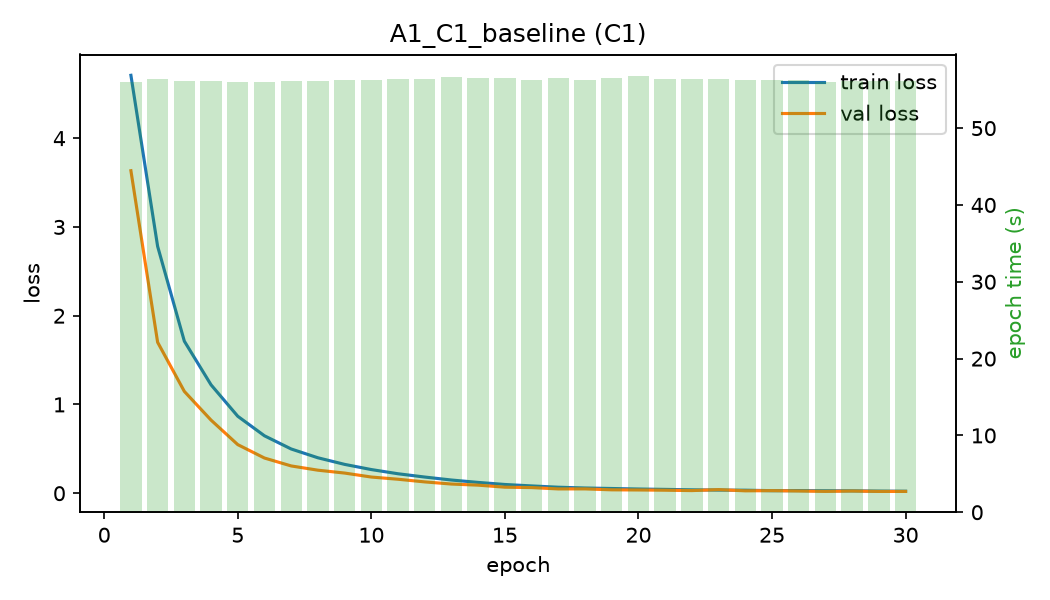
\includegraphics[width=\textwidth]{outputs/plots/A1_C1_baseline_curves.png}
        \caption{C1: Baseline}
    \end{subfigure}
    \hfill
    \begin{subfigure}[b]{0.32\textwidth}
        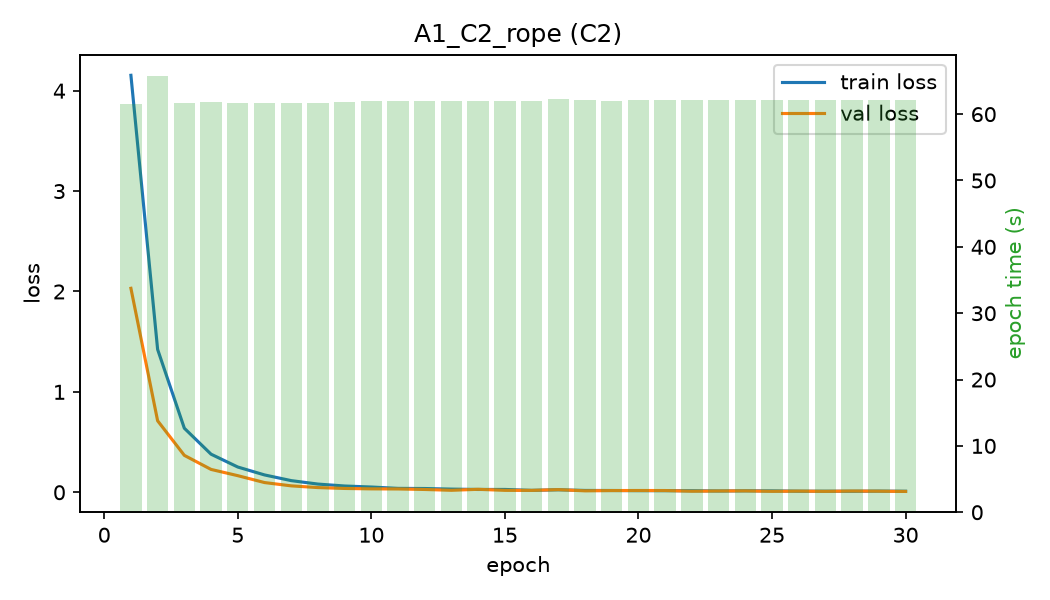
\includegraphics[width=\textwidth]{outputs/plots/A1_C2_rope_curves.png}
        \caption{C2: RoPE}
    \end{subfigure}
    \hfill
    \begin{subfigure}[b]{0.32\textwidth}
        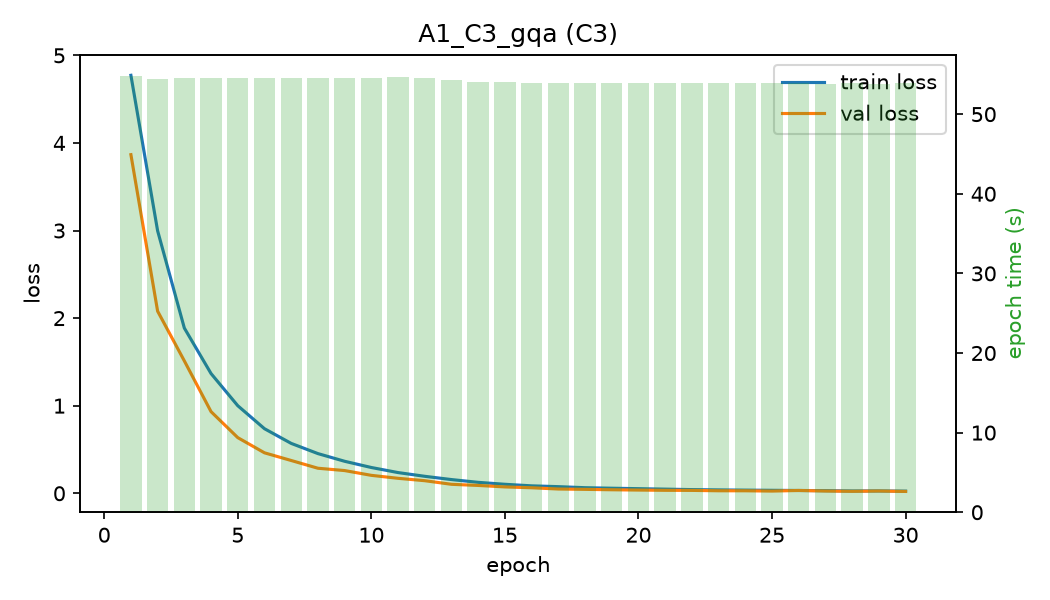
\includegraphics[width=\textwidth]{outputs/plots/A1_C3_gqa_curves.png}
        \caption{C3: GQA}
    \end{subfigure}
    \par\vspace{0.4em}
    \begin{subfigure}[b]{0.32\textwidth}
        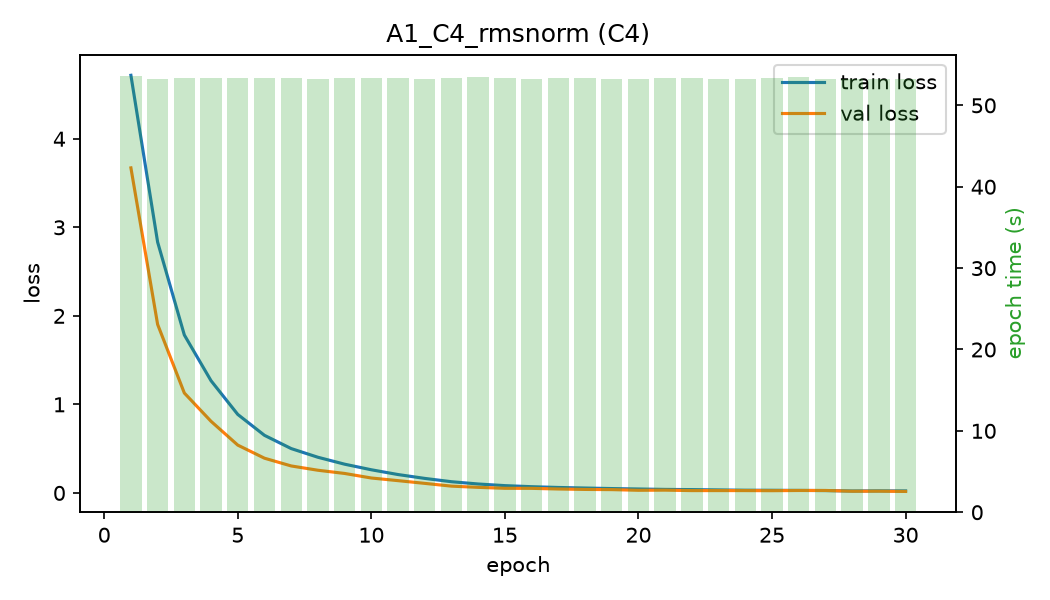
\includegraphics[width=\textwidth]{outputs/plots/A1_C4_rmsnorm_curves.png}
        \caption{C4: RMSNorm}
    \end{subfigure}
    \qquad
    \begin{subfigure}[b]{0.32\textwidth}
        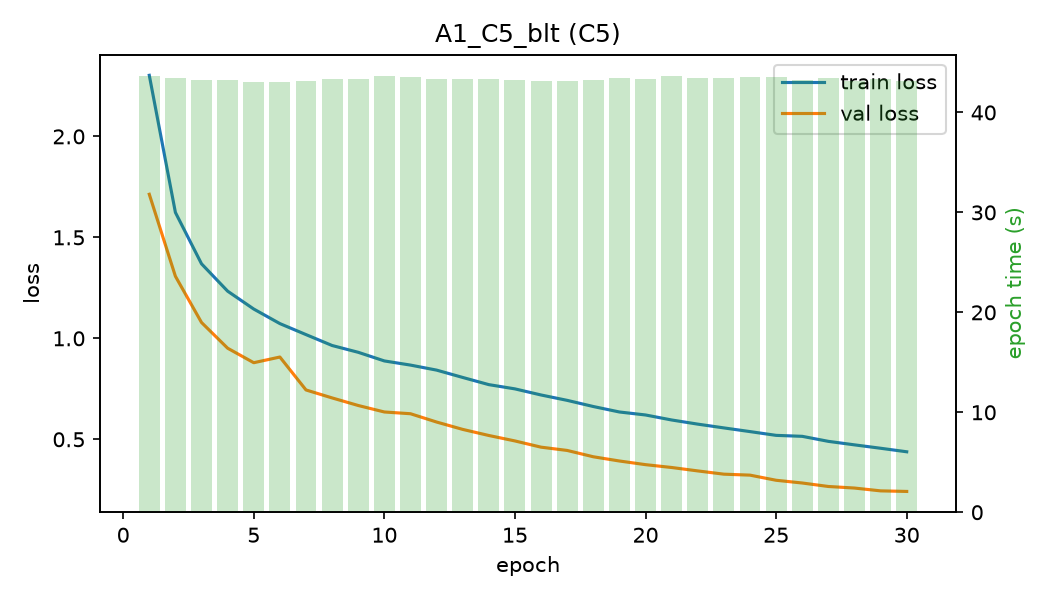
\includegraphics[width=\textwidth]{outputs/plots/A1_C5_blt_curves.png}
        \caption{C5: BLT (Token-Free)}
    \end{subfigure}
    \caption{\textbf{Training and Validation Loss Curves} across all 30 epochs.}
    \label{fig:curves}
\end{figure}

\section{Byte Latent Transformer (C5)}

\subsection{Advantages of BLT: Memory and Speed}
Because standard self-attention scales quadratically with sequence length, compressing 64 bytes into just 4 patches ($P=16$) basically decreases a lot of memory requirement.
\begin{itemize}
    \item C5 used only \textbf{$608.31\,\text{MB}$} of VRAM, compared to \textbf{$1212.15\,\text{MB}$} for C1.
    \item \textbf{23\% Faster Training:} C5 finished 30 epochs in just \textbf{$1306.09\,\text{s}$}.
\end{itemize}

\subsection{The Catch: Compounding Errors and Accuracy Drops}
Despite the massive compute savings, C5's accuracy tanked compared to the baseline. It got $84.15\%$ bit accuracy, but a brutal $3.48\%$ exact sequence match. When you look at the actual text it generates, you can see exactly what's going wrong:
\begin{quote}
\small
\textbf{Ref:} \texttt{'Credits adapted from the Loose liner notes'} \\
\textbf{Pred:} \texttt{'Cradisted topearfrom the Loose liner tones'} \\
\textbf{Ref:} \texttt{'In January the embassy arrived at Beijing and was received by th'} \\
\textbf{Pred:} \texttt{'In January the embassary reviduat Minge a was fis received by th'}
\end{quote}
The model is clearly learning English syntax and figuring out the cipher patterns, but it completely fails at exact sequence matching for two main reasons ( I think ) :
\begin{enumerate}
    \item \textbf{Compounding Error over 64 Steps:} The C1 model only has to decode about 18 BPE tokens per chunk. C5 has to decode 64 individual bytes in a row perfectly. Even if it gets $98\%$ accuracy on every single step, $0.98^{64}$ gives you terrible odds of getting the whole sequence right. Just one wrong character ruins the sequence match metric.
    \item \textbf{Fixed 16-Byte Patching is Clunky:} Meta's original paper uses dynamic patching to cleanly split text at word boundaries. Because I only used a fixed $P=16$ patch size, the 16-byte boundaries blindly bisect words and morphemes across patch cuts. Compressing these disjoint character fragments into one vector makes it much harder for the local decoder to reconstruct fluent, error-free words from scratch.
\end{enumerate}

\end{document}